\apendice{Especificación de diseño}

\section{Introducción}
En esta sección se detallan los aspectos más importantes de la aplicación: los datos utilizados, los procedimientos de la aplicación, la arquitectura de la aplicación y el diseño de las interfaces.

\section{Diseño de datos}
Los datos utilizados para el desarrollo de la aplicación no quedan más allá del almacenamiento de los usuarios en una base de datos y el procesamiento del vídeo.

Dado que la aplicación desarrollada cuenta con alta, modificación y baja de usuarios, así como la obligación de estar dado de alta para utilizar la aplicación, esta debe estar conectada con una base de datos para almacenar los datos de los usuarios. La base de datos cuenta con una única tabla donde se almacena la información de los usuarios agregados, siguiendo la siguiente estructura de columnas:

\begin{itemize}
	\item \textbf{id:} es el identificador único del usuario. En la base de datos es una clave primaria.
	\item \textbf{usuario:} es el nombre de usuario que se utilizará para iniciar sesión. Debe ser único para cada usuario, por lo que en la base de datos es un UNIQUE.
	\item \textbf{contraseña:} es la contraseña utilizada para iniciar sesión junto al usuario correspondiente. Dado que la contraseña debe ser secreta, en la base de datos se guarda encriptada.
	\item \textbf{nombre\_completo:} es el nombre completo del usuario. Su utilidad es dar la bienvenida al usuario que inicie sesión en la aplicación.
\end{itemize}

Para realizar la predicción, se debe procesar el vídeo subido al servidor. Los datos obtenidos para predecir son los mismos que se utilizaron en la fase de investigación. Estos son: las amplitudes normalizadas, la velocidad media, la mano y el sexo. Una vez obtenidas las características, se utilizan en el modelo entrenado previamente para realizar la predicción.

\section{Diseño procedimental}

\section{Diseño arquitectónico}

\section{Diseño de interfaces}
En este apartado, se muestran los diseños realizados de la aplicación web con la función de mostrar las funcionalidades que tendría la aplicación web, además de mostrar una interfaz con aspecto amigable.

\subsection{Vista de usuario}
Las pantallas del usuario son idénticas a las del administrador con la diferencia de que los usuarios no tendrán las opciones de ``Gestionar usuarios'' y ``Modificar modelo'', en su lugar tendrán la opción ``Modificar usuario''. Además, tendrán ventanas restringidas a las que únicamente el usuario administrador podrá acceder. Las ventanas disponibles para los usuarios sin privilegios son las correspondientes a las figuras \ref{fig:inicio_de_sesion}, \ref{fig:inicio}, \ref{fig:resultado} y \ref{fig:modificar_usuario}.

\subsection{Vista de administrador}
Se muestra el diseño de las interfaces para un usuario con privilegios.
\begin{figure}[h]
	\frame{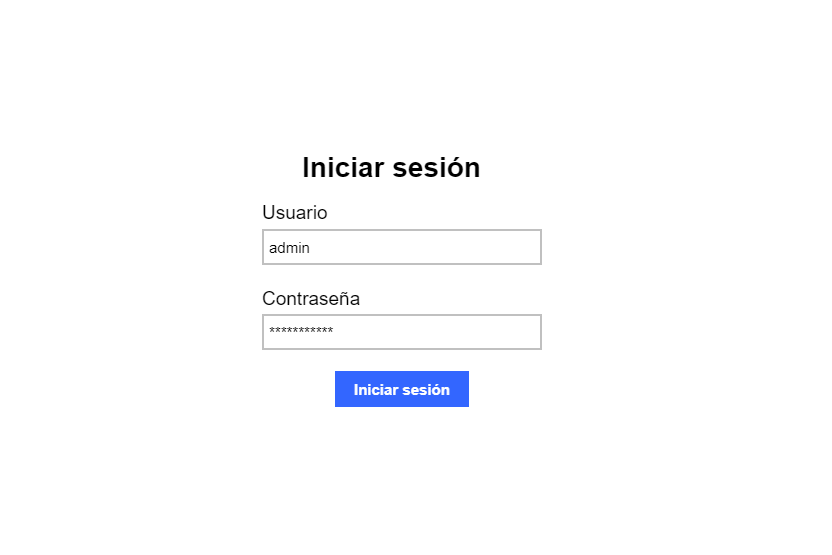
\includegraphics[width=1\textwidth]{inicio_de_sesion_admin}}
	\caption{Pantalla de inicio de sesión de un usuario administrador.}
	\label{fig:inicio_de_sesion}
\end{figure}

\begin{figure}[h]
	\frame{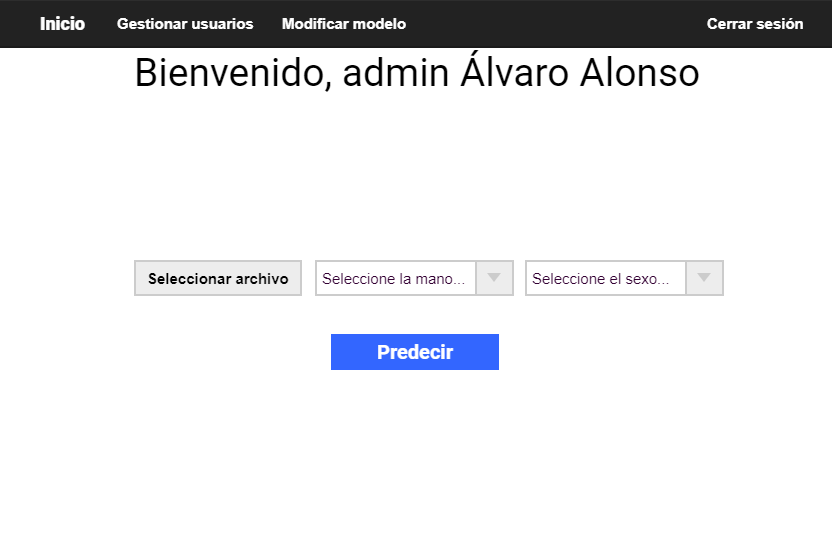
\includegraphics[width=1\textwidth]{inicio_admin}}
	\caption{Pantalla inicial de un usuario administrador.}
	\label{fig:inicio}
\end{figure}

\begin{figure}[h]
	\frame{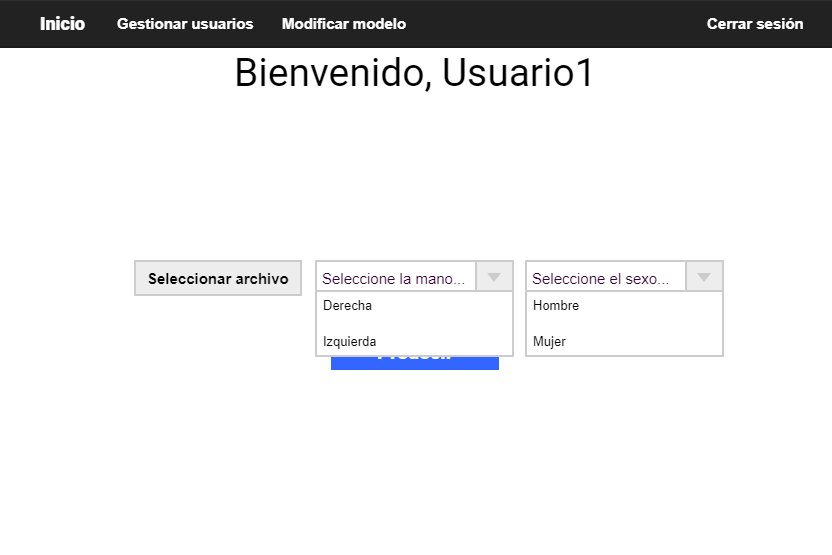
\includegraphics[width=1\textwidth]{inicio_admin_1}}
	\caption{Pantalla inicial de un usuario administrador con las listas desplegadas.}
	\label{fig:inicio_1}
\end{figure}

\begin{figure}[h]
	\frame{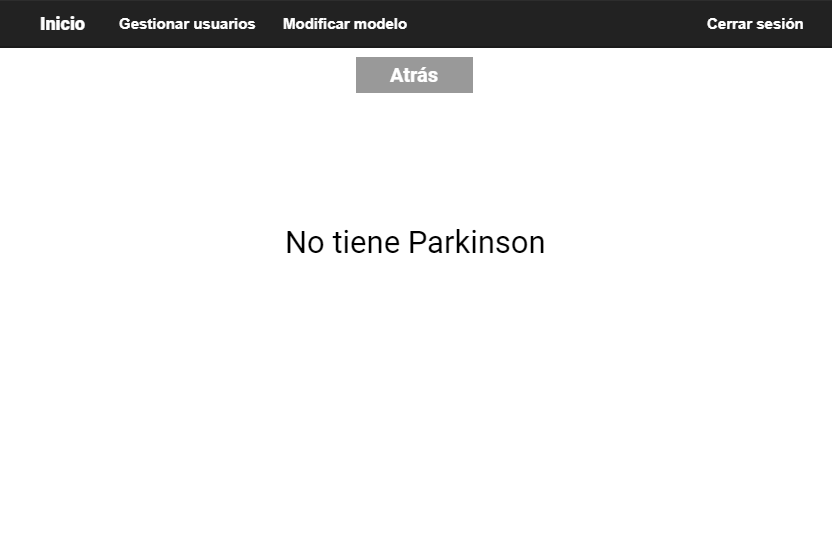
\includegraphics[width=1\textwidth]{resultado_admin}}
	\caption{Pantalla con el resultado de la predicción de un usuario administrador.}
	\label{fig:resultado}
\end{figure}

\begin{figure}[h]
	\frame{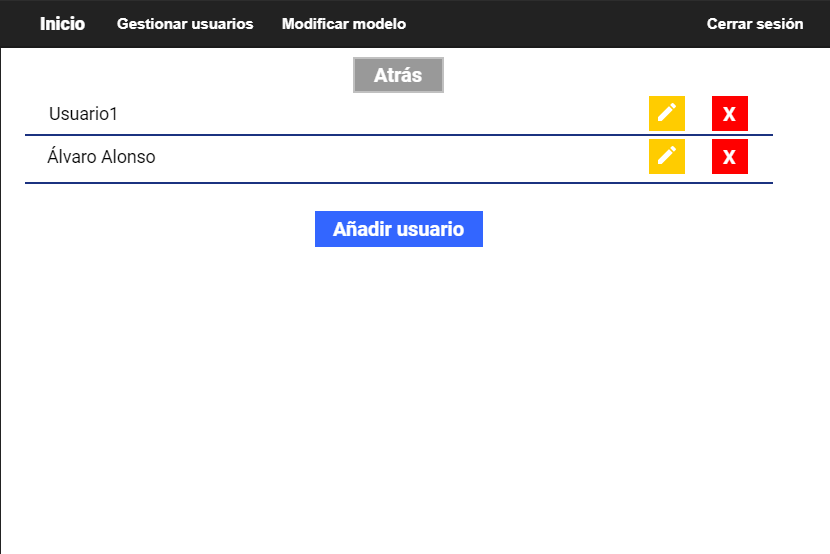
\includegraphics[width=1\textwidth]{gestionar_usuarios}}
	\caption{Pantalla con el listado de los usuarios dados de alta en la aplicación.}
	\label{fig:gestionar_usuarios}
\end{figure}

\begin{figure}[h]
	\frame{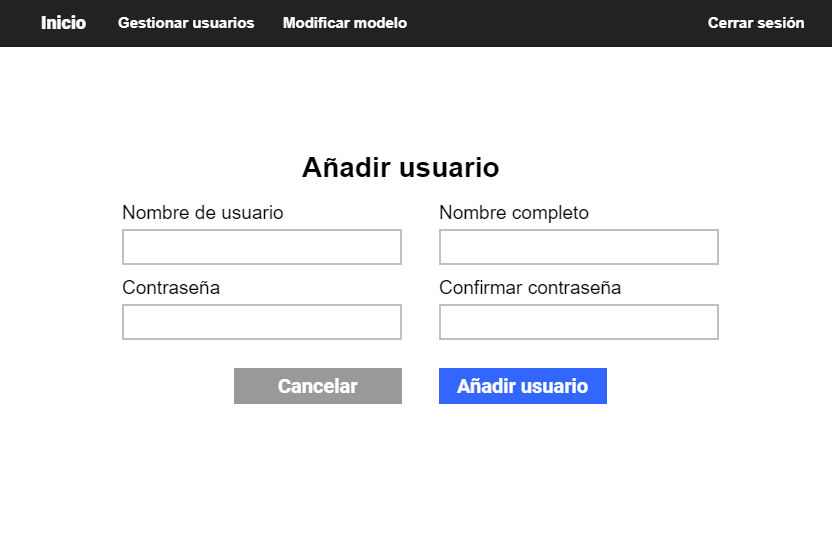
\includegraphics[width=1\textwidth]{agregar_usuario}}
	\caption{Pantalla con el formulario para dar de alta a un usuario.}
	\label{fig:agregar_usuario}
\end{figure}

\begin{figure}[h]
	\frame{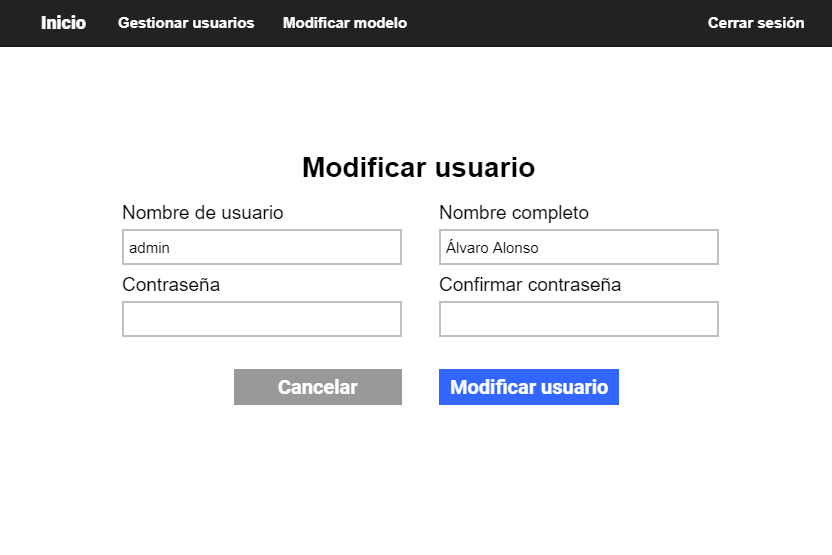
\includegraphics[width=1\textwidth]{modificar_usuario}}
	\caption{Pantalla con el formulario para modificar un usuario existente.}
	\label{fig:modificar_usuario}
\end{figure}

\begin{figure}[h]
	\frame{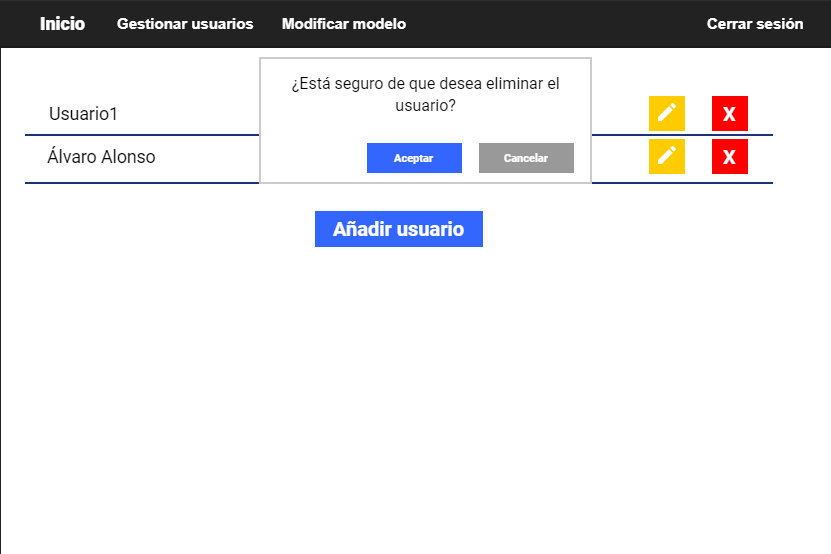
\includegraphics[width=1\textwidth]{eliminar_usuario}}
	\caption{Pantalla con la confirmación para borrar el usuario.}
	\label{fig:eliminar_usuario}
\end{figure}

\begin{figure}[h]
	\frame{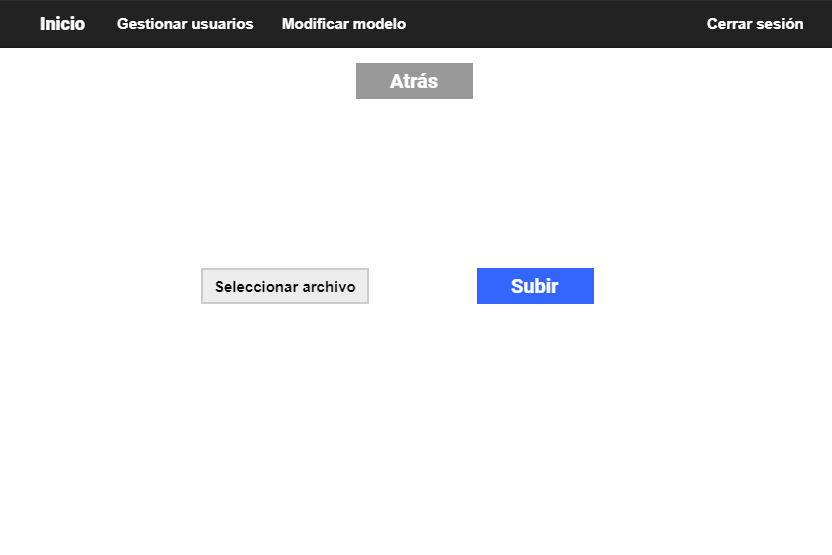
\includegraphics[width=1\textwidth]{modificar_modelo}}
	\caption{Pantalla con la subida del modelo al servidor.}
	\label{fig:modificar_modelo}
\end{figure}
